% Standalone wrapper to rebuild figures/blocked_likelihood.pdf
% from blocked_likelihood_tikz.tex.
%
% Why this exists: the figure is included into ms.tex as a pre-rendered PDF
% rather than via % blocked_likelihood_tikz.tex
%
% Schematic of the blocked, coarse-grained periodogram pipeline.
\usetikzlibrary{arrows.meta, calc, positioning, decorations.pathreplacing}
%
% Use as: % blocked_likelihood_tikz.tex
%
% Schematic of the blocked, coarse-grained periodogram pipeline.
\usetikzlibrary{arrows.meta, calc, positioning, decorations.pathreplacing}
%
% Use as: % blocked_likelihood_tikz.tex
%
% Schematic of the blocked, coarse-grained periodogram pipeline.
\usetikzlibrary{arrows.meta, calc, positioning, decorations.pathreplacing}
%
% Use as: \input{blocked_likelihood_tikz}
%
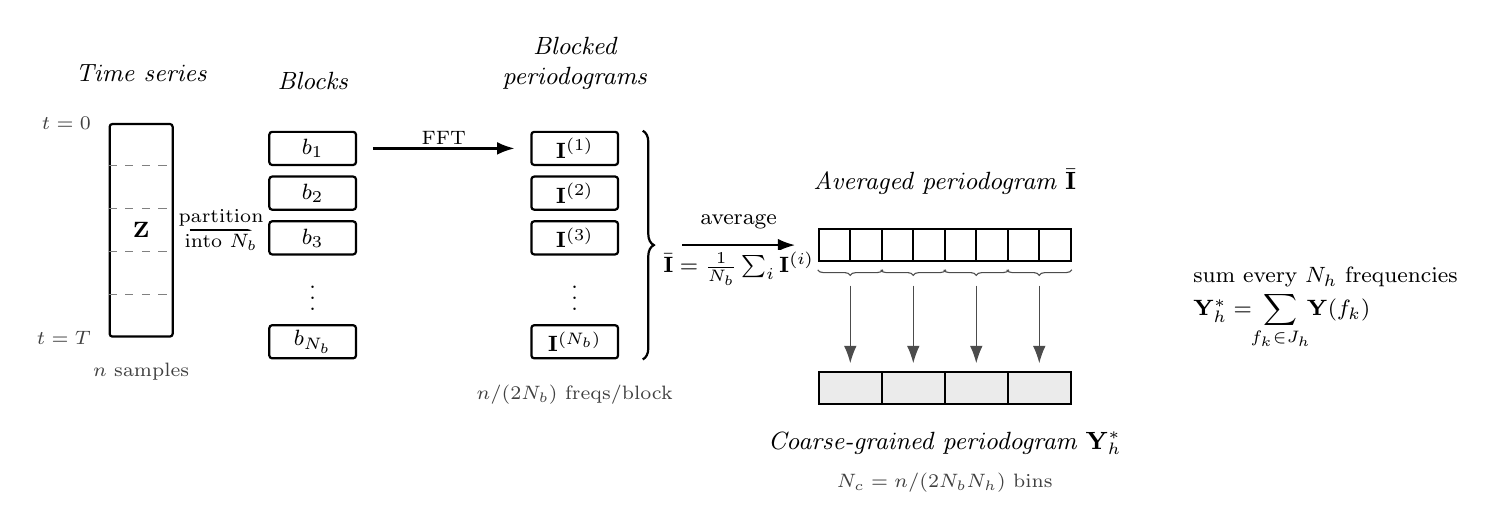
\begin{tikzpicture}[
    >={Latex[length=2.2mm,width=1.6mm]},
    font=\footnotesize,
    block/.style={draw, thick, rounded corners=1pt,
                  minimum width=11mm, minimum height=4.2mm,
                  inner sep=1pt, fill=white},
    cell/.style={draw, thick,
                 minimum width=4mm, minimum height=4mm,
                 inner sep=0pt, fill=white},
    coarsecell/.style={draw, thick,
                 minimum width=8mm, minimum height=4mm,
                 inner sep=0pt, fill=black!8},
    stagelabel/.style={font=\small\itshape, align=center},
    lengthlabel/.style={font=\scriptsize, align=center, text=black!75},
    arrowlabel/.style={font=\scriptsize, align=center,
                       fill=white, inner sep=1pt},
    formulalabel/.style={font=\footnotesize, align=center,
                       fill=white, inner sep=1pt},
]

% ---------------- Stage 0: full timeseries Z ----------------------------
% Single tall rectangle with internal dashed lines indicating block edges.
\node[draw, thick, rounded corners=1pt,
      minimum width=8mm, minimum height=27mm,
      inner sep=0pt, fill=white]                  (Z)     at (0, -3) {$\Z$};

% Dashed lines inside Z marking block boundaries (4 dashes for 5 blocks).
\foreach \frac in {0.2, 0.4, 0.6, 0.8} {%
    \draw[dashed, black!50]
        ($(Z.north west)!\frac!(Z.south west)$) --
        ($(Z.north east)!\frac!(Z.south east)$);
}

\node[stagelabel, above=4mm of Z.north]
    {Time series};
\node[lengthlabel, below=2mm of Z.south]
    {$n$ samples};
\node[lengthlabel, left=1mm of Z.north west]   {$t=0$};
\node[lengthlabel, left=1mm of Z.south west]   {$t=T$};

% ---------------- Stage 1: blocks (vertical stack) ----------------------
\node[block, right=12mm of Z.east, yshift=10.4mm] (b1)    {$b_1$};
\node[block, below=1.2mm of b1]                   (b2)    {$b_2$};
\node[block, below=1.2mm of b2]                   (b3)    {$b_3$};
\node[below=0.5mm of b3]                          (bdots) {$\vdots$};
\node[block, below=0.5mm of bdots]                (bNb)   {$b_{N_{b}}$};

\node[stagelabel, above=4mm of b1.north]
    {Blocks};

% Arrow: Z -> blocks (partitioning step)
\draw[->, thick] ([xshift=2mm]Z.east) -- ([xshift=-2mm]b1.west |- Z.east)
    node[arrowlabel, midway, above]{partition}
    node[arrowlabel, midway, below]{into $N_b$};

% ---------------- Stage 2: blocked periodograms -------------------------
\node[block, right=22mm of b1]    (p1)    {$\mathbf{I}^{(1)}$};
\node[block, below=1.2mm of p1]   (p2)    {$\mathbf{I}^{(2)}$};
\node[block, below=1.2mm of p2]   (p3)    {$\mathbf{I}^{(3)}$};
\node[below=0.5mm of p3]          (pdots) {$\vdots$};
\node[block, below=0.5mm of pdots] (pNb)  {$\mathbf{I}^{(N_{b})}$};

\node[stagelabel, above=4mm of p1.north]
    {Blocked\\periodograms};
\node[lengthlabel, below=2mm of pNb.south]
    {$n/(2N_{b})$ freqs/block};

% Arrow stage1 -> stage2
\draw[->, thick] ([xshift=2mm]b1.east) -- ([xshift=-2mm]p1.west)
    node[arrowlabel, midway, above]{FFT};

% Brace gathering all blocked periodograms
\draw[decorate, decoration={brace, amplitude=4pt}, thick]
    ([xshift=3mm]p1.north east) -- ([xshift=3mm]pNb.south east);

% Arrow stage2 -> stage3 with averaging formula
\coordinate (braceTip) at ($(p1.east)!0.5!(pNb.east) + (8mm, 0)$);
\coordinate (avgcenter) at ($(p1)!0.5!(pNb) + (47mm, 0)$);
\coordinate (avgLeft)   at ($(avgcenter) + (-19mm, 0)$);

\draw[->, thick] (braceTip) -- (avgLeft);
\node[formulalabel] at ($(braceTip)!0.5!(avgLeft) + (0, 3mm)$)
    {average};
\node[formulalabel] at ($(braceTip)!0.5!(avgLeft) + (0, -3mm)$)
    {$\bar{\mathbf{I}}=\tfrac{1}{N_{b}}\sum_{i}\mathbf{I}^{(i)}$};

% ---------------- Stage 3: averaged periodogram (8 fine cells) ----------
\foreach \i in {1,...,8} {%
    \node[cell] at ($(avgcenter) + ({(\i-4.5)*4mm}, 0)$) (avg\i) {};
}

\node[stagelabel] at ($(avgcenter) + (0, 8mm)$)
    {Averaged periodogram $\bar{\mathbf{I}}$};

% ---------------- Stage 4: coarse-grained periodogram (4 cells) ---------
% Coarse cells one row below, with each centred on a pair of fine cells.
\foreach \i [evaluate=\i as \k using int(2*\i-1)] in {1,...,4} {%
    \node[coarsecell]
        at ($(avg\k.south)!0.5!(avg\the\numexpr\k+1\relax.south)
            + (0, -16mm)$) (cg\i) {};
}

% Small braces under each pair of fine cells, pointing to the coarse cell.
\foreach \i [evaluate=\i as \k using int(2*\i-1)] in {1,...,4} {%
    \draw[decorate, decoration={brace, amplitude=2pt, mirror},
          thin, black!70]
        ([yshift=-1mm]avg\k.south west) --
        ([yshift=-1mm]avg\the\numexpr\k+1\relax.south east);
    \draw[->, thin, black!70]
        ($(avg\k.south)!0.5!(avg\the\numexpr\k+1\relax.south) + (0, -3mm)$)
        -- ([yshift=1mm]cg\i.north);
}

% Stage 4 stage label below the coarse cells
\node[stagelabel] at ($(cg1)!0.5!(cg4) + (0, -7mm)$)
    {Coarse-grained periodogram $\mathbf{Y}_{h}^{*}$};
\node[lengthlabel] at ($(cg1)!0.5!(cg4) + (0, -12mm)$)
    {$N_{c}=n/(2N_{b}N_{h})$ bins};

% Side caption to the right explaining the grouping operation.
\node[formulalabel, anchor=west, align=left]
    at ($(avg8.east) + (15mm, -8mm)$)
    {sum every $N_{h}$ frequencies\\[1pt]
     $\mathbf{Y}_{h}^{*}=\!\!\displaystyle\sum_{f_{k}\in J_{h}}\!\!\mathbf{Y}(f_{k})$};

\end{tikzpicture}

%
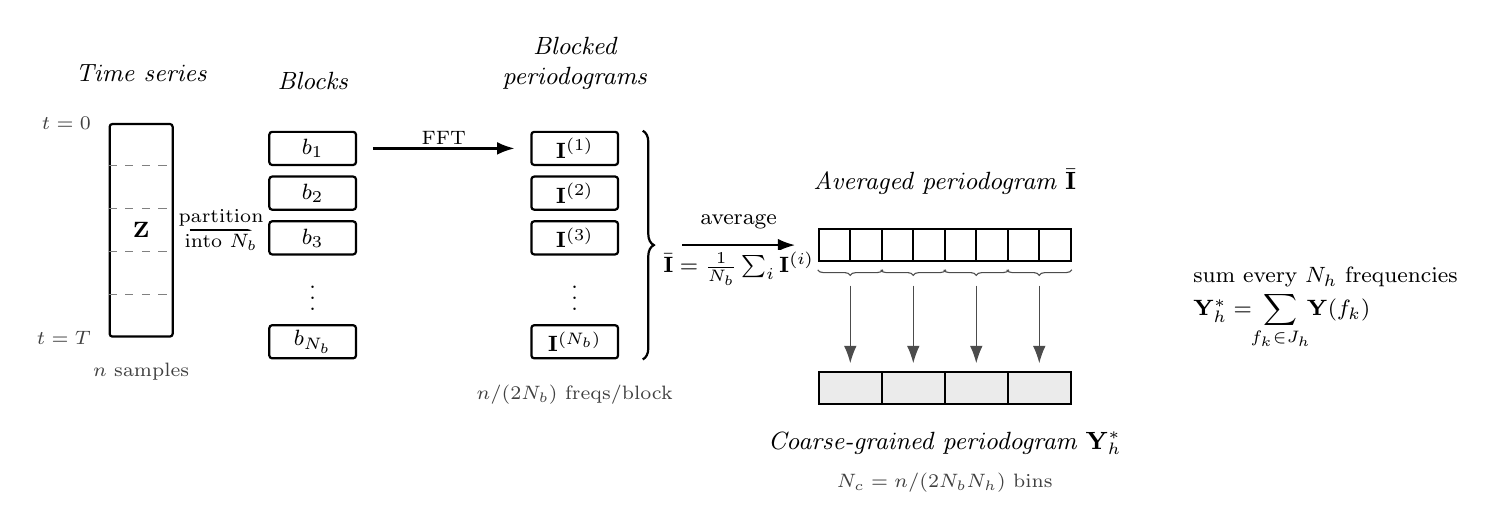
\begin{tikzpicture}[
    >={Latex[length=2.2mm,width=1.6mm]},
    font=\footnotesize,
    block/.style={draw, thick, rounded corners=1pt,
                  minimum width=11mm, minimum height=4.2mm,
                  inner sep=1pt, fill=white},
    cell/.style={draw, thick,
                 minimum width=4mm, minimum height=4mm,
                 inner sep=0pt, fill=white},
    coarsecell/.style={draw, thick,
                 minimum width=8mm, minimum height=4mm,
                 inner sep=0pt, fill=black!8},
    stagelabel/.style={font=\small\itshape, align=center},
    lengthlabel/.style={font=\scriptsize, align=center, text=black!75},
    arrowlabel/.style={font=\scriptsize, align=center,
                       fill=white, inner sep=1pt},
    formulalabel/.style={font=\footnotesize, align=center,
                       fill=white, inner sep=1pt},
]

% ---------------- Stage 0: full timeseries Z ----------------------------
% Single tall rectangle with internal dashed lines indicating block edges.
\node[draw, thick, rounded corners=1pt,
      minimum width=8mm, minimum height=27mm,
      inner sep=0pt, fill=white]                  (Z)     at (0, -3) {$\Z$};

% Dashed lines inside Z marking block boundaries (4 dashes for 5 blocks).
\foreach \frac in {0.2, 0.4, 0.6, 0.8} {%
    \draw[dashed, black!50]
        ($(Z.north west)!\frac!(Z.south west)$) --
        ($(Z.north east)!\frac!(Z.south east)$);
}

\node[stagelabel, above=4mm of Z.north]
    {Time series};
\node[lengthlabel, below=2mm of Z.south]
    {$n$ samples};
\node[lengthlabel, left=1mm of Z.north west]   {$t=0$};
\node[lengthlabel, left=1mm of Z.south west]   {$t=T$};

% ---------------- Stage 1: blocks (vertical stack) ----------------------
\node[block, right=12mm of Z.east, yshift=10.4mm] (b1)    {$b_1$};
\node[block, below=1.2mm of b1]                   (b2)    {$b_2$};
\node[block, below=1.2mm of b2]                   (b3)    {$b_3$};
\node[below=0.5mm of b3]                          (bdots) {$\vdots$};
\node[block, below=0.5mm of bdots]                (bNb)   {$b_{N_{b}}$};

\node[stagelabel, above=4mm of b1.north]
    {Blocks};

% Arrow: Z -> blocks (partitioning step)
\draw[->, thick] ([xshift=2mm]Z.east) -- ([xshift=-2mm]b1.west |- Z.east)
    node[arrowlabel, midway, above]{partition}
    node[arrowlabel, midway, below]{into $N_b$};

% ---------------- Stage 2: blocked periodograms -------------------------
\node[block, right=22mm of b1]    (p1)    {$\mathbf{I}^{(1)}$};
\node[block, below=1.2mm of p1]   (p2)    {$\mathbf{I}^{(2)}$};
\node[block, below=1.2mm of p2]   (p3)    {$\mathbf{I}^{(3)}$};
\node[below=0.5mm of p3]          (pdots) {$\vdots$};
\node[block, below=0.5mm of pdots] (pNb)  {$\mathbf{I}^{(N_{b})}$};

\node[stagelabel, above=4mm of p1.north]
    {Blocked\\periodograms};
\node[lengthlabel, below=2mm of pNb.south]
    {$n/(2N_{b})$ freqs/block};

% Arrow stage1 -> stage2
\draw[->, thick] ([xshift=2mm]b1.east) -- ([xshift=-2mm]p1.west)
    node[arrowlabel, midway, above]{FFT};

% Brace gathering all blocked periodograms
\draw[decorate, decoration={brace, amplitude=4pt}, thick]
    ([xshift=3mm]p1.north east) -- ([xshift=3mm]pNb.south east);

% Arrow stage2 -> stage3 with averaging formula
\coordinate (braceTip) at ($(p1.east)!0.5!(pNb.east) + (8mm, 0)$);
\coordinate (avgcenter) at ($(p1)!0.5!(pNb) + (47mm, 0)$);
\coordinate (avgLeft)   at ($(avgcenter) + (-19mm, 0)$);

\draw[->, thick] (braceTip) -- (avgLeft);
\node[formulalabel] at ($(braceTip)!0.5!(avgLeft) + (0, 3mm)$)
    {average};
\node[formulalabel] at ($(braceTip)!0.5!(avgLeft) + (0, -3mm)$)
    {$\bar{\mathbf{I}}=\tfrac{1}{N_{b}}\sum_{i}\mathbf{I}^{(i)}$};

% ---------------- Stage 3: averaged periodogram (8 fine cells) ----------
\foreach \i in {1,...,8} {%
    \node[cell] at ($(avgcenter) + ({(\i-4.5)*4mm}, 0)$) (avg\i) {};
}

\node[stagelabel] at ($(avgcenter) + (0, 8mm)$)
    {Averaged periodogram $\bar{\mathbf{I}}$};

% ---------------- Stage 4: coarse-grained periodogram (4 cells) ---------
% Coarse cells one row below, with each centred on a pair of fine cells.
\foreach \i [evaluate=\i as \k using int(2*\i-1)] in {1,...,4} {%
    \node[coarsecell]
        at ($(avg\k.south)!0.5!(avg\the\numexpr\k+1\relax.south)
            + (0, -16mm)$) (cg\i) {};
}

% Small braces under each pair of fine cells, pointing to the coarse cell.
\foreach \i [evaluate=\i as \k using int(2*\i-1)] in {1,...,4} {%
    \draw[decorate, decoration={brace, amplitude=2pt, mirror},
          thin, black!70]
        ([yshift=-1mm]avg\k.south west) --
        ([yshift=-1mm]avg\the\numexpr\k+1\relax.south east);
    \draw[->, thin, black!70]
        ($(avg\k.south)!0.5!(avg\the\numexpr\k+1\relax.south) + (0, -3mm)$)
        -- ([yshift=1mm]cg\i.north);
}

% Stage 4 stage label below the coarse cells
\node[stagelabel] at ($(cg1)!0.5!(cg4) + (0, -7mm)$)
    {Coarse-grained periodogram $\mathbf{Y}_{h}^{*}$};
\node[lengthlabel] at ($(cg1)!0.5!(cg4) + (0, -12mm)$)
    {$N_{c}=n/(2N_{b}N_{h})$ bins};

% Side caption to the right explaining the grouping operation.
\node[formulalabel, anchor=west, align=left]
    at ($(avg8.east) + (15mm, -8mm)$)
    {sum every $N_{h}$ frequencies\\[1pt]
     $\mathbf{Y}_{h}^{*}=\!\!\displaystyle\sum_{f_{k}\in J_{h}}\!\!\mathbf{Y}(f_{k})$};

\end{tikzpicture}

%
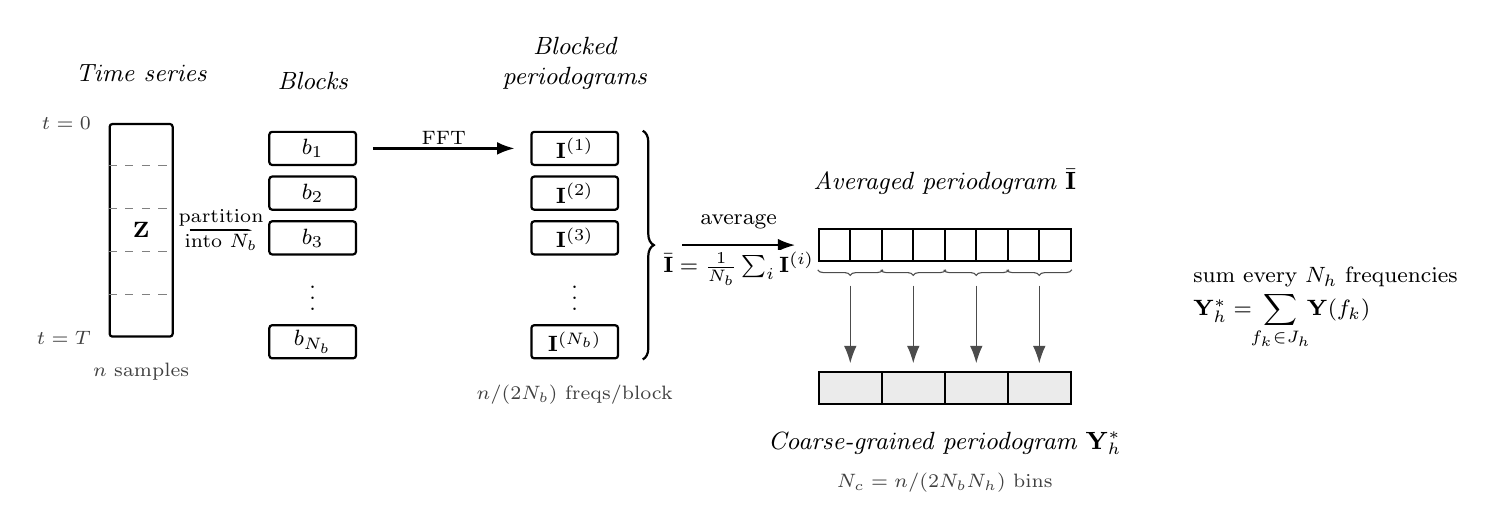
\begin{tikzpicture}[
    >={Latex[length=2.2mm,width=1.6mm]},
    font=\footnotesize,
    block/.style={draw, thick, rounded corners=1pt,
                  minimum width=11mm, minimum height=4.2mm,
                  inner sep=1pt, fill=white},
    cell/.style={draw, thick,
                 minimum width=4mm, minimum height=4mm,
                 inner sep=0pt, fill=white},
    coarsecell/.style={draw, thick,
                 minimum width=8mm, minimum height=4mm,
                 inner sep=0pt, fill=black!8},
    stagelabel/.style={font=\small\itshape, align=center},
    lengthlabel/.style={font=\scriptsize, align=center, text=black!75},
    arrowlabel/.style={font=\scriptsize, align=center,
                       fill=white, inner sep=1pt},
    formulalabel/.style={font=\footnotesize, align=center,
                       fill=white, inner sep=1pt},
]

% ---------------- Stage 0: full timeseries Z ----------------------------
% Single tall rectangle with internal dashed lines indicating block edges.
\node[draw, thick, rounded corners=1pt,
      minimum width=8mm, minimum height=27mm,
      inner sep=0pt, fill=white]                  (Z)     at (0, -3) {$\Z$};

% Dashed lines inside Z marking block boundaries (4 dashes for 5 blocks).
\foreach \frac in {0.2, 0.4, 0.6, 0.8} {%
    \draw[dashed, black!50]
        ($(Z.north west)!\frac!(Z.south west)$) --
        ($(Z.north east)!\frac!(Z.south east)$);
}

\node[stagelabel, above=4mm of Z.north]
    {Time series};
\node[lengthlabel, below=2mm of Z.south]
    {$n$ samples};
\node[lengthlabel, left=1mm of Z.north west]   {$t=0$};
\node[lengthlabel, left=1mm of Z.south west]   {$t=T$};

% ---------------- Stage 1: blocks (vertical stack) ----------------------
\node[block, right=12mm of Z.east, yshift=10.4mm] (b1)    {$b_1$};
\node[block, below=1.2mm of b1]                   (b2)    {$b_2$};
\node[block, below=1.2mm of b2]                   (b3)    {$b_3$};
\node[below=0.5mm of b3]                          (bdots) {$\vdots$};
\node[block, below=0.5mm of bdots]                (bNb)   {$b_{N_{b}}$};

\node[stagelabel, above=4mm of b1.north]
    {Blocks};

% Arrow: Z -> blocks (partitioning step)
\draw[->, thick] ([xshift=2mm]Z.east) -- ([xshift=-2mm]b1.west |- Z.east)
    node[arrowlabel, midway, above]{partition}
    node[arrowlabel, midway, below]{into $N_b$};

% ---------------- Stage 2: blocked periodograms -------------------------
\node[block, right=22mm of b1]    (p1)    {$\mathbf{I}^{(1)}$};
\node[block, below=1.2mm of p1]   (p2)    {$\mathbf{I}^{(2)}$};
\node[block, below=1.2mm of p2]   (p3)    {$\mathbf{I}^{(3)}$};
\node[below=0.5mm of p3]          (pdots) {$\vdots$};
\node[block, below=0.5mm of pdots] (pNb)  {$\mathbf{I}^{(N_{b})}$};

\node[stagelabel, above=4mm of p1.north]
    {Blocked\\periodograms};
\node[lengthlabel, below=2mm of pNb.south]
    {$n/(2N_{b})$ freqs/block};

% Arrow stage1 -> stage2
\draw[->, thick] ([xshift=2mm]b1.east) -- ([xshift=-2mm]p1.west)
    node[arrowlabel, midway, above]{FFT};

% Brace gathering all blocked periodograms
\draw[decorate, decoration={brace, amplitude=4pt}, thick]
    ([xshift=3mm]p1.north east) -- ([xshift=3mm]pNb.south east);

% Arrow stage2 -> stage3 with averaging formula
\coordinate (braceTip) at ($(p1.east)!0.5!(pNb.east) + (8mm, 0)$);
\coordinate (avgcenter) at ($(p1)!0.5!(pNb) + (47mm, 0)$);
\coordinate (avgLeft)   at ($(avgcenter) + (-19mm, 0)$);

\draw[->, thick] (braceTip) -- (avgLeft);
\node[formulalabel] at ($(braceTip)!0.5!(avgLeft) + (0, 3mm)$)
    {average};
\node[formulalabel] at ($(braceTip)!0.5!(avgLeft) + (0, -3mm)$)
    {$\bar{\mathbf{I}}=\tfrac{1}{N_{b}}\sum_{i}\mathbf{I}^{(i)}$};

% ---------------- Stage 3: averaged periodogram (8 fine cells) ----------
\foreach \i in {1,...,8} {%
    \node[cell] at ($(avgcenter) + ({(\i-4.5)*4mm}, 0)$) (avg\i) {};
}

\node[stagelabel] at ($(avgcenter) + (0, 8mm)$)
    {Averaged periodogram $\bar{\mathbf{I}}$};

% ---------------- Stage 4: coarse-grained periodogram (4 cells) ---------
% Coarse cells one row below, with each centred on a pair of fine cells.
\foreach \i [evaluate=\i as \k using int(2*\i-1)] in {1,...,4} {%
    \node[coarsecell]
        at ($(avg\k.south)!0.5!(avg\the\numexpr\k+1\relax.south)
            + (0, -16mm)$) (cg\i) {};
}

% Small braces under each pair of fine cells, pointing to the coarse cell.
\foreach \i [evaluate=\i as \k using int(2*\i-1)] in {1,...,4} {%
    \draw[decorate, decoration={brace, amplitude=2pt, mirror},
          thin, black!70]
        ([yshift=-1mm]avg\k.south west) --
        ([yshift=-1mm]avg\the\numexpr\k+1\relax.south east);
    \draw[->, thin, black!70]
        ($(avg\k.south)!0.5!(avg\the\numexpr\k+1\relax.south) + (0, -3mm)$)
        -- ([yshift=1mm]cg\i.north);
}

% Stage 4 stage label below the coarse cells
\node[stagelabel] at ($(cg1)!0.5!(cg4) + (0, -7mm)$)
    {Coarse-grained periodogram $\mathbf{Y}_{h}^{*}$};
\node[lengthlabel] at ($(cg1)!0.5!(cg4) + (0, -12mm)$)
    {$N_{c}=n/(2N_{b}N_{h})$ bins};

% Side caption to the right explaining the grouping operation.
\node[formulalabel, anchor=west, align=left]
    at ($(avg8.east) + (15mm, -8mm)$)
    {sum every $N_{h}$ frequencies\\[1pt]
     $\mathbf{Y}_{h}^{*}=\!\!\displaystyle\sum_{f_{k}\in J_{h}}\!\!\mathbf{Y}(f_{k})$};

\end{tikzpicture}
, because Overleaf's
% free-tier compile budget can time out on the live TikZ render.
%
% Rebuild (run from src/tex/):
%     tectonic build_blocked_likelihood.tex
%     mv build_blocked_likelihood.pdf figures/blocked_likelihood.pdf
%
% (pdflatex works too: `pdflatex build_blocked_likelihood.tex`.)
%
% The \newcommand block below mirrors the math macros that ms.tex defines
% in its preamble -- keep them in sync if you add new symbols to the figure.

\documentclass[tikz,border=2pt]{standalone}
\usepackage{tikz}
\usepackage{amsmath,amssymb,bm}
\usetikzlibrary{arrows.meta, calc, positioning, decorations.pathreplacing}

\newcommand{\Z}{{\bf Z}}
\newcommand{\Y}{{\bf Y}}
\renewcommand{\S}{{\bf S}}
\renewcommand{\d}{{\bf d}}
\newcommand{\I}{\mbox{{\bf I}}}

\begin{document}
% blocked_likelihood_tikz.tex
%
% Schematic of the blocked, coarse-grained periodogram pipeline.
\usetikzlibrary{arrows.meta, calc, positioning, decorations.pathreplacing}
%
% Use as: % blocked_likelihood_tikz.tex
%
% Schematic of the blocked, coarse-grained periodogram pipeline.
\usetikzlibrary{arrows.meta, calc, positioning, decorations.pathreplacing}
%
% Use as: % blocked_likelihood_tikz.tex
%
% Schematic of the blocked, coarse-grained periodogram pipeline.
\usetikzlibrary{arrows.meta, calc, positioning, decorations.pathreplacing}
%
% Use as: \input{blocked_likelihood_tikz}
%
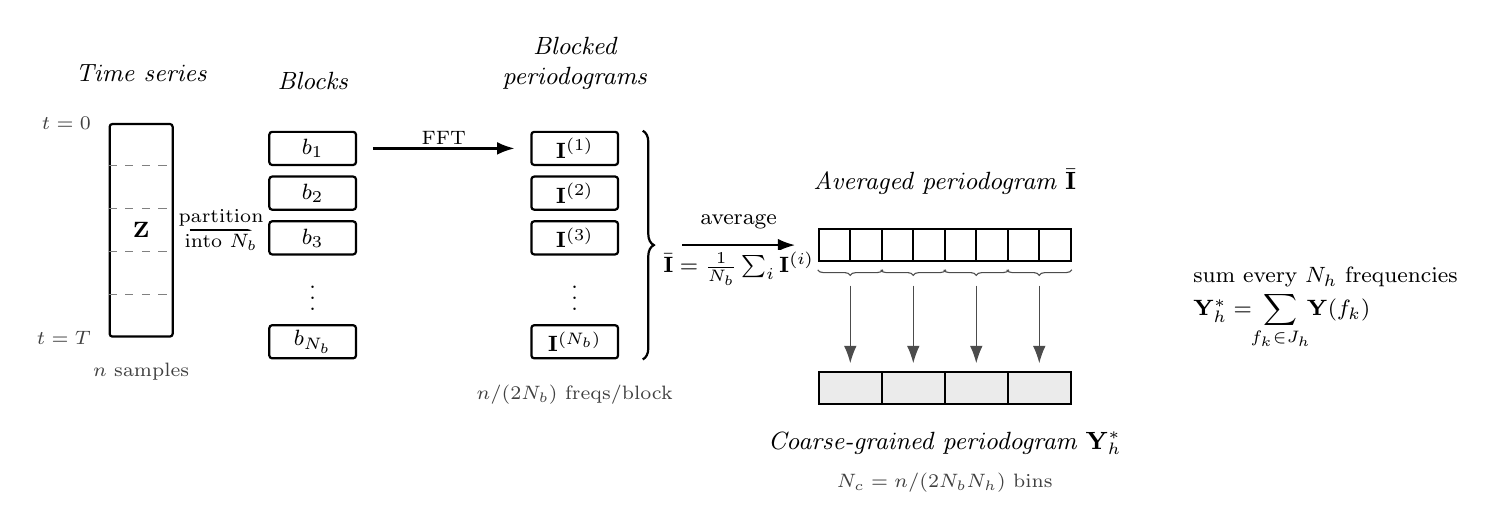
\begin{tikzpicture}[
    >={Latex[length=2.2mm,width=1.6mm]},
    font=\footnotesize,
    block/.style={draw, thick, rounded corners=1pt,
                  minimum width=11mm, minimum height=4.2mm,
                  inner sep=1pt, fill=white},
    cell/.style={draw, thick,
                 minimum width=4mm, minimum height=4mm,
                 inner sep=0pt, fill=white},
    coarsecell/.style={draw, thick,
                 minimum width=8mm, minimum height=4mm,
                 inner sep=0pt, fill=black!8},
    stagelabel/.style={font=\small\itshape, align=center},
    lengthlabel/.style={font=\scriptsize, align=center, text=black!75},
    arrowlabel/.style={font=\scriptsize, align=center,
                       fill=white, inner sep=1pt},
    formulalabel/.style={font=\footnotesize, align=center,
                       fill=white, inner sep=1pt},
]

% ---------------- Stage 0: full timeseries Z ----------------------------
% Single tall rectangle with internal dashed lines indicating block edges.
\node[draw, thick, rounded corners=1pt,
      minimum width=8mm, minimum height=27mm,
      inner sep=0pt, fill=white]                  (Z)     at (0, -3) {$\Z$};

% Dashed lines inside Z marking block boundaries (4 dashes for 5 blocks).
\foreach \frac in {0.2, 0.4, 0.6, 0.8} {%
    \draw[dashed, black!50]
        ($(Z.north west)!\frac!(Z.south west)$) --
        ($(Z.north east)!\frac!(Z.south east)$);
}

\node[stagelabel, above=4mm of Z.north]
    {Time series};
\node[lengthlabel, below=2mm of Z.south]
    {$n$ samples};
\node[lengthlabel, left=1mm of Z.north west]   {$t=0$};
\node[lengthlabel, left=1mm of Z.south west]   {$t=T$};

% ---------------- Stage 1: blocks (vertical stack) ----------------------
\node[block, right=12mm of Z.east, yshift=10.4mm] (b1)    {$b_1$};
\node[block, below=1.2mm of b1]                   (b2)    {$b_2$};
\node[block, below=1.2mm of b2]                   (b3)    {$b_3$};
\node[below=0.5mm of b3]                          (bdots) {$\vdots$};
\node[block, below=0.5mm of bdots]                (bNb)   {$b_{N_{b}}$};

\node[stagelabel, above=4mm of b1.north]
    {Blocks};

% Arrow: Z -> blocks (partitioning step)
\draw[->, thick] ([xshift=2mm]Z.east) -- ([xshift=-2mm]b1.west |- Z.east)
    node[arrowlabel, midway, above]{partition}
    node[arrowlabel, midway, below]{into $N_b$};

% ---------------- Stage 2: blocked periodograms -------------------------
\node[block, right=22mm of b1]    (p1)    {$\mathbf{I}^{(1)}$};
\node[block, below=1.2mm of p1]   (p2)    {$\mathbf{I}^{(2)}$};
\node[block, below=1.2mm of p2]   (p3)    {$\mathbf{I}^{(3)}$};
\node[below=0.5mm of p3]          (pdots) {$\vdots$};
\node[block, below=0.5mm of pdots] (pNb)  {$\mathbf{I}^{(N_{b})}$};

\node[stagelabel, above=4mm of p1.north]
    {Blocked\\periodograms};
\node[lengthlabel, below=2mm of pNb.south]
    {$n/(2N_{b})$ freqs/block};

% Arrow stage1 -> stage2
\draw[->, thick] ([xshift=2mm]b1.east) -- ([xshift=-2mm]p1.west)
    node[arrowlabel, midway, above]{FFT};

% Brace gathering all blocked periodograms
\draw[decorate, decoration={brace, amplitude=4pt}, thick]
    ([xshift=3mm]p1.north east) -- ([xshift=3mm]pNb.south east);

% Arrow stage2 -> stage3 with averaging formula
\coordinate (braceTip) at ($(p1.east)!0.5!(pNb.east) + (8mm, 0)$);
\coordinate (avgcenter) at ($(p1)!0.5!(pNb) + (47mm, 0)$);
\coordinate (avgLeft)   at ($(avgcenter) + (-19mm, 0)$);

\draw[->, thick] (braceTip) -- (avgLeft);
\node[formulalabel] at ($(braceTip)!0.5!(avgLeft) + (0, 3mm)$)
    {average};
\node[formulalabel] at ($(braceTip)!0.5!(avgLeft) + (0, -3mm)$)
    {$\bar{\mathbf{I}}=\tfrac{1}{N_{b}}\sum_{i}\mathbf{I}^{(i)}$};

% ---------------- Stage 3: averaged periodogram (8 fine cells) ----------
\foreach \i in {1,...,8} {%
    \node[cell] at ($(avgcenter) + ({(\i-4.5)*4mm}, 0)$) (avg\i) {};
}

\node[stagelabel] at ($(avgcenter) + (0, 8mm)$)
    {Averaged periodogram $\bar{\mathbf{I}}$};

% ---------------- Stage 4: coarse-grained periodogram (4 cells) ---------
% Coarse cells one row below, with each centred on a pair of fine cells.
\foreach \i [evaluate=\i as \k using int(2*\i-1)] in {1,...,4} {%
    \node[coarsecell]
        at ($(avg\k.south)!0.5!(avg\the\numexpr\k+1\relax.south)
            + (0, -16mm)$) (cg\i) {};
}

% Small braces under each pair of fine cells, pointing to the coarse cell.
\foreach \i [evaluate=\i as \k using int(2*\i-1)] in {1,...,4} {%
    \draw[decorate, decoration={brace, amplitude=2pt, mirror},
          thin, black!70]
        ([yshift=-1mm]avg\k.south west) --
        ([yshift=-1mm]avg\the\numexpr\k+1\relax.south east);
    \draw[->, thin, black!70]
        ($(avg\k.south)!0.5!(avg\the\numexpr\k+1\relax.south) + (0, -3mm)$)
        -- ([yshift=1mm]cg\i.north);
}

% Stage 4 stage label below the coarse cells
\node[stagelabel] at ($(cg1)!0.5!(cg4) + (0, -7mm)$)
    {Coarse-grained periodogram $\mathbf{Y}_{h}^{*}$};
\node[lengthlabel] at ($(cg1)!0.5!(cg4) + (0, -12mm)$)
    {$N_{c}=n/(2N_{b}N_{h})$ bins};

% Side caption to the right explaining the grouping operation.
\node[formulalabel, anchor=west, align=left]
    at ($(avg8.east) + (15mm, -8mm)$)
    {sum every $N_{h}$ frequencies\\[1pt]
     $\mathbf{Y}_{h}^{*}=\!\!\displaystyle\sum_{f_{k}\in J_{h}}\!\!\mathbf{Y}(f_{k})$};

\end{tikzpicture}

%
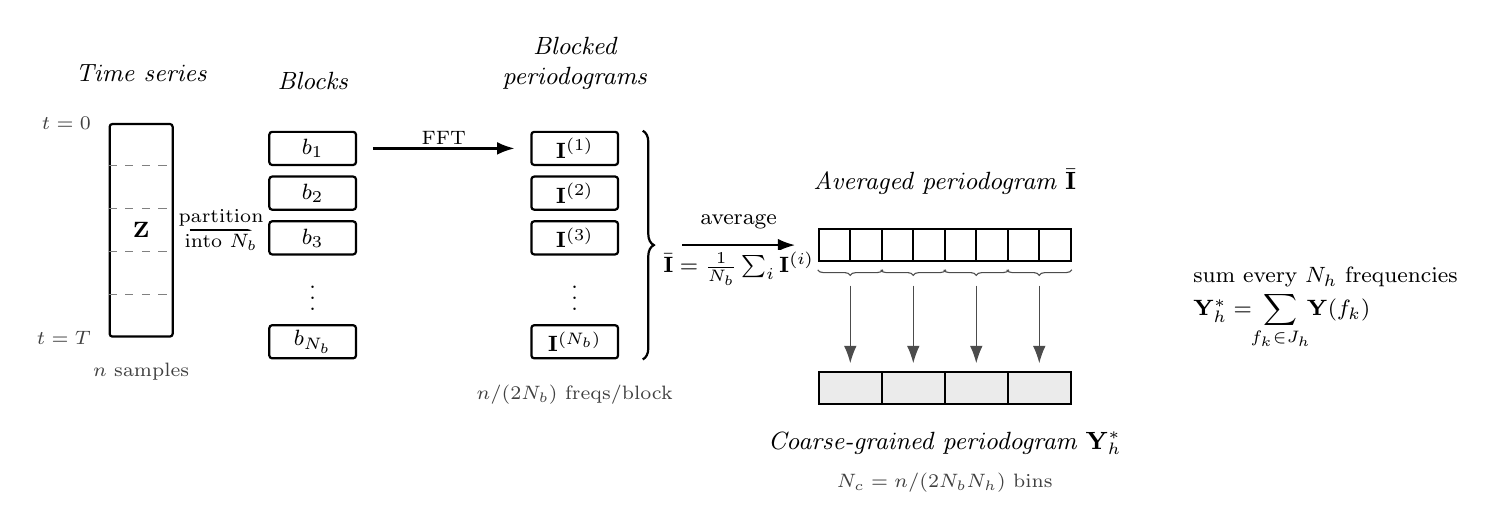
\begin{tikzpicture}[
    >={Latex[length=2.2mm,width=1.6mm]},
    font=\footnotesize,
    block/.style={draw, thick, rounded corners=1pt,
                  minimum width=11mm, minimum height=4.2mm,
                  inner sep=1pt, fill=white},
    cell/.style={draw, thick,
                 minimum width=4mm, minimum height=4mm,
                 inner sep=0pt, fill=white},
    coarsecell/.style={draw, thick,
                 minimum width=8mm, minimum height=4mm,
                 inner sep=0pt, fill=black!8},
    stagelabel/.style={font=\small\itshape, align=center},
    lengthlabel/.style={font=\scriptsize, align=center, text=black!75},
    arrowlabel/.style={font=\scriptsize, align=center,
                       fill=white, inner sep=1pt},
    formulalabel/.style={font=\footnotesize, align=center,
                       fill=white, inner sep=1pt},
]

% ---------------- Stage 0: full timeseries Z ----------------------------
% Single tall rectangle with internal dashed lines indicating block edges.
\node[draw, thick, rounded corners=1pt,
      minimum width=8mm, minimum height=27mm,
      inner sep=0pt, fill=white]                  (Z)     at (0, -3) {$\Z$};

% Dashed lines inside Z marking block boundaries (4 dashes for 5 blocks).
\foreach \frac in {0.2, 0.4, 0.6, 0.8} {%
    \draw[dashed, black!50]
        ($(Z.north west)!\frac!(Z.south west)$) --
        ($(Z.north east)!\frac!(Z.south east)$);
}

\node[stagelabel, above=4mm of Z.north]
    {Time series};
\node[lengthlabel, below=2mm of Z.south]
    {$n$ samples};
\node[lengthlabel, left=1mm of Z.north west]   {$t=0$};
\node[lengthlabel, left=1mm of Z.south west]   {$t=T$};

% ---------------- Stage 1: blocks (vertical stack) ----------------------
\node[block, right=12mm of Z.east, yshift=10.4mm] (b1)    {$b_1$};
\node[block, below=1.2mm of b1]                   (b2)    {$b_2$};
\node[block, below=1.2mm of b2]                   (b3)    {$b_3$};
\node[below=0.5mm of b3]                          (bdots) {$\vdots$};
\node[block, below=0.5mm of bdots]                (bNb)   {$b_{N_{b}}$};

\node[stagelabel, above=4mm of b1.north]
    {Blocks};

% Arrow: Z -> blocks (partitioning step)
\draw[->, thick] ([xshift=2mm]Z.east) -- ([xshift=-2mm]b1.west |- Z.east)
    node[arrowlabel, midway, above]{partition}
    node[arrowlabel, midway, below]{into $N_b$};

% ---------------- Stage 2: blocked periodograms -------------------------
\node[block, right=22mm of b1]    (p1)    {$\mathbf{I}^{(1)}$};
\node[block, below=1.2mm of p1]   (p2)    {$\mathbf{I}^{(2)}$};
\node[block, below=1.2mm of p2]   (p3)    {$\mathbf{I}^{(3)}$};
\node[below=0.5mm of p3]          (pdots) {$\vdots$};
\node[block, below=0.5mm of pdots] (pNb)  {$\mathbf{I}^{(N_{b})}$};

\node[stagelabel, above=4mm of p1.north]
    {Blocked\\periodograms};
\node[lengthlabel, below=2mm of pNb.south]
    {$n/(2N_{b})$ freqs/block};

% Arrow stage1 -> stage2
\draw[->, thick] ([xshift=2mm]b1.east) -- ([xshift=-2mm]p1.west)
    node[arrowlabel, midway, above]{FFT};

% Brace gathering all blocked periodograms
\draw[decorate, decoration={brace, amplitude=4pt}, thick]
    ([xshift=3mm]p1.north east) -- ([xshift=3mm]pNb.south east);

% Arrow stage2 -> stage3 with averaging formula
\coordinate (braceTip) at ($(p1.east)!0.5!(pNb.east) + (8mm, 0)$);
\coordinate (avgcenter) at ($(p1)!0.5!(pNb) + (47mm, 0)$);
\coordinate (avgLeft)   at ($(avgcenter) + (-19mm, 0)$);

\draw[->, thick] (braceTip) -- (avgLeft);
\node[formulalabel] at ($(braceTip)!0.5!(avgLeft) + (0, 3mm)$)
    {average};
\node[formulalabel] at ($(braceTip)!0.5!(avgLeft) + (0, -3mm)$)
    {$\bar{\mathbf{I}}=\tfrac{1}{N_{b}}\sum_{i}\mathbf{I}^{(i)}$};

% ---------------- Stage 3: averaged periodogram (8 fine cells) ----------
\foreach \i in {1,...,8} {%
    \node[cell] at ($(avgcenter) + ({(\i-4.5)*4mm}, 0)$) (avg\i) {};
}

\node[stagelabel] at ($(avgcenter) + (0, 8mm)$)
    {Averaged periodogram $\bar{\mathbf{I}}$};

% ---------------- Stage 4: coarse-grained periodogram (4 cells) ---------
% Coarse cells one row below, with each centred on a pair of fine cells.
\foreach \i [evaluate=\i as \k using int(2*\i-1)] in {1,...,4} {%
    \node[coarsecell]
        at ($(avg\k.south)!0.5!(avg\the\numexpr\k+1\relax.south)
            + (0, -16mm)$) (cg\i) {};
}

% Small braces under each pair of fine cells, pointing to the coarse cell.
\foreach \i [evaluate=\i as \k using int(2*\i-1)] in {1,...,4} {%
    \draw[decorate, decoration={brace, amplitude=2pt, mirror},
          thin, black!70]
        ([yshift=-1mm]avg\k.south west) --
        ([yshift=-1mm]avg\the\numexpr\k+1\relax.south east);
    \draw[->, thin, black!70]
        ($(avg\k.south)!0.5!(avg\the\numexpr\k+1\relax.south) + (0, -3mm)$)
        -- ([yshift=1mm]cg\i.north);
}

% Stage 4 stage label below the coarse cells
\node[stagelabel] at ($(cg1)!0.5!(cg4) + (0, -7mm)$)
    {Coarse-grained periodogram $\mathbf{Y}_{h}^{*}$};
\node[lengthlabel] at ($(cg1)!0.5!(cg4) + (0, -12mm)$)
    {$N_{c}=n/(2N_{b}N_{h})$ bins};

% Side caption to the right explaining the grouping operation.
\node[formulalabel, anchor=west, align=left]
    at ($(avg8.east) + (15mm, -8mm)$)
    {sum every $N_{h}$ frequencies\\[1pt]
     $\mathbf{Y}_{h}^{*}=\!\!\displaystyle\sum_{f_{k}\in J_{h}}\!\!\mathbf{Y}(f_{k})$};

\end{tikzpicture}

%
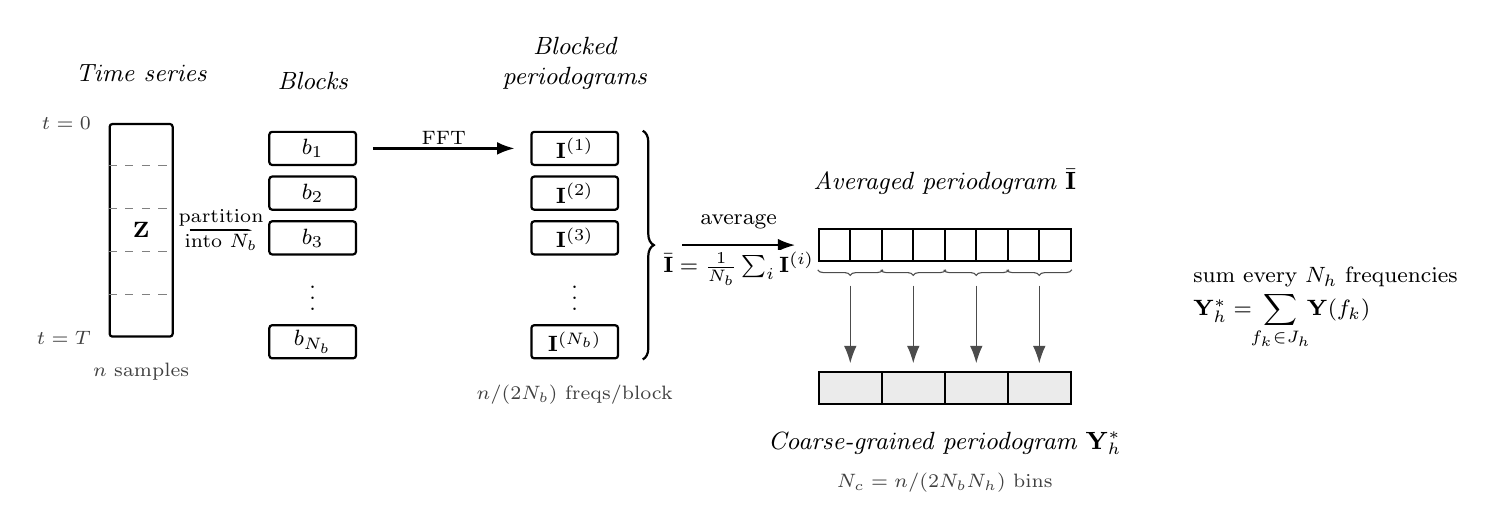
\begin{tikzpicture}[
    >={Latex[length=2.2mm,width=1.6mm]},
    font=\footnotesize,
    block/.style={draw, thick, rounded corners=1pt,
                  minimum width=11mm, minimum height=4.2mm,
                  inner sep=1pt, fill=white},
    cell/.style={draw, thick,
                 minimum width=4mm, minimum height=4mm,
                 inner sep=0pt, fill=white},
    coarsecell/.style={draw, thick,
                 minimum width=8mm, minimum height=4mm,
                 inner sep=0pt, fill=black!8},
    stagelabel/.style={font=\small\itshape, align=center},
    lengthlabel/.style={font=\scriptsize, align=center, text=black!75},
    arrowlabel/.style={font=\scriptsize, align=center,
                       fill=white, inner sep=1pt},
    formulalabel/.style={font=\footnotesize, align=center,
                       fill=white, inner sep=1pt},
]

% ---------------- Stage 0: full timeseries Z ----------------------------
% Single tall rectangle with internal dashed lines indicating block edges.
\node[draw, thick, rounded corners=1pt,
      minimum width=8mm, minimum height=27mm,
      inner sep=0pt, fill=white]                  (Z)     at (0, -3) {$\Z$};

% Dashed lines inside Z marking block boundaries (4 dashes for 5 blocks).
\foreach \frac in {0.2, 0.4, 0.6, 0.8} {%
    \draw[dashed, black!50]
        ($(Z.north west)!\frac!(Z.south west)$) --
        ($(Z.north east)!\frac!(Z.south east)$);
}

\node[stagelabel, above=4mm of Z.north]
    {Time series};
\node[lengthlabel, below=2mm of Z.south]
    {$n$ samples};
\node[lengthlabel, left=1mm of Z.north west]   {$t=0$};
\node[lengthlabel, left=1mm of Z.south west]   {$t=T$};

% ---------------- Stage 1: blocks (vertical stack) ----------------------
\node[block, right=12mm of Z.east, yshift=10.4mm] (b1)    {$b_1$};
\node[block, below=1.2mm of b1]                   (b2)    {$b_2$};
\node[block, below=1.2mm of b2]                   (b3)    {$b_3$};
\node[below=0.5mm of b3]                          (bdots) {$\vdots$};
\node[block, below=0.5mm of bdots]                (bNb)   {$b_{N_{b}}$};

\node[stagelabel, above=4mm of b1.north]
    {Blocks};

% Arrow: Z -> blocks (partitioning step)
\draw[->, thick] ([xshift=2mm]Z.east) -- ([xshift=-2mm]b1.west |- Z.east)
    node[arrowlabel, midway, above]{partition}
    node[arrowlabel, midway, below]{into $N_b$};

% ---------------- Stage 2: blocked periodograms -------------------------
\node[block, right=22mm of b1]    (p1)    {$\mathbf{I}^{(1)}$};
\node[block, below=1.2mm of p1]   (p2)    {$\mathbf{I}^{(2)}$};
\node[block, below=1.2mm of p2]   (p3)    {$\mathbf{I}^{(3)}$};
\node[below=0.5mm of p3]          (pdots) {$\vdots$};
\node[block, below=0.5mm of pdots] (pNb)  {$\mathbf{I}^{(N_{b})}$};

\node[stagelabel, above=4mm of p1.north]
    {Blocked\\periodograms};
\node[lengthlabel, below=2mm of pNb.south]
    {$n/(2N_{b})$ freqs/block};

% Arrow stage1 -> stage2
\draw[->, thick] ([xshift=2mm]b1.east) -- ([xshift=-2mm]p1.west)
    node[arrowlabel, midway, above]{FFT};

% Brace gathering all blocked periodograms
\draw[decorate, decoration={brace, amplitude=4pt}, thick]
    ([xshift=3mm]p1.north east) -- ([xshift=3mm]pNb.south east);

% Arrow stage2 -> stage3 with averaging formula
\coordinate (braceTip) at ($(p1.east)!0.5!(pNb.east) + (8mm, 0)$);
\coordinate (avgcenter) at ($(p1)!0.5!(pNb) + (47mm, 0)$);
\coordinate (avgLeft)   at ($(avgcenter) + (-19mm, 0)$);

\draw[->, thick] (braceTip) -- (avgLeft);
\node[formulalabel] at ($(braceTip)!0.5!(avgLeft) + (0, 3mm)$)
    {average};
\node[formulalabel] at ($(braceTip)!0.5!(avgLeft) + (0, -3mm)$)
    {$\bar{\mathbf{I}}=\tfrac{1}{N_{b}}\sum_{i}\mathbf{I}^{(i)}$};

% ---------------- Stage 3: averaged periodogram (8 fine cells) ----------
\foreach \i in {1,...,8} {%
    \node[cell] at ($(avgcenter) + ({(\i-4.5)*4mm}, 0)$) (avg\i) {};
}

\node[stagelabel] at ($(avgcenter) + (0, 8mm)$)
    {Averaged periodogram $\bar{\mathbf{I}}$};

% ---------------- Stage 4: coarse-grained periodogram (4 cells) ---------
% Coarse cells one row below, with each centred on a pair of fine cells.
\foreach \i [evaluate=\i as \k using int(2*\i-1)] in {1,...,4} {%
    \node[coarsecell]
        at ($(avg\k.south)!0.5!(avg\the\numexpr\k+1\relax.south)
            + (0, -16mm)$) (cg\i) {};
}

% Small braces under each pair of fine cells, pointing to the coarse cell.
\foreach \i [evaluate=\i as \k using int(2*\i-1)] in {1,...,4} {%
    \draw[decorate, decoration={brace, amplitude=2pt, mirror},
          thin, black!70]
        ([yshift=-1mm]avg\k.south west) --
        ([yshift=-1mm]avg\the\numexpr\k+1\relax.south east);
    \draw[->, thin, black!70]
        ($(avg\k.south)!0.5!(avg\the\numexpr\k+1\relax.south) + (0, -3mm)$)
        -- ([yshift=1mm]cg\i.north);
}

% Stage 4 stage label below the coarse cells
\node[stagelabel] at ($(cg1)!0.5!(cg4) + (0, -7mm)$)
    {Coarse-grained periodogram $\mathbf{Y}_{h}^{*}$};
\node[lengthlabel] at ($(cg1)!0.5!(cg4) + (0, -12mm)$)
    {$N_{c}=n/(2N_{b}N_{h})$ bins};

% Side caption to the right explaining the grouping operation.
\node[formulalabel, anchor=west, align=left]
    at ($(avg8.east) + (15mm, -8mm)$)
    {sum every $N_{h}$ frequencies\\[1pt]
     $\mathbf{Y}_{h}^{*}=\!\!\displaystyle\sum_{f_{k}\in J_{h}}\!\!\mathbf{Y}(f_{k})$};

\end{tikzpicture}

\end{document}
